\noindent \textit{brass prismatical-box,}\edtext{}{\lemma{\textit{prismatical-box},}\Cfootnote{a.a.O., S. 64.}} et eam cementabam \textit{very tight, with hard and soft Ciment}\edtext{}{\lemma{\textit{Ciment}}\Cfootnote{a.a.O., S. 64.}}. Habebat \textit{the plate}\edtext{}{\lemma{\textit{plate}}\Cfootnote{a.a.O., S. 64.}} (frustum, lamina) curvum canalem, \textit{ground in it in the length thereof}\edtext{}{\lemma{\textit{thereof}}\Cfootnote{a.a.O., S. 64.}} aptum ad servandam in medio bullam. Horum mediorum ope non est difficile tendere seu curvare hanc laminam seu tabulam in circulum 50, 60, 100, 1000 pedum radiorum, \textit{and the Brass Box can easily be made to fill or empty, as there shall be occasion for the use thereof, so that the bubble may be at any time left, of what bigness shall be desired. It will be convenient also, to varnish the inside of this brass-box, with laker-varnish, very thik and close, }\edtext{\textit{both to keep it from}}{\lemma{\textit{close},}\Bfootnote{\textit{(1)}\ tum ut \textit{(2)}\ \textit{both to keep it from} \textit{L}}} \textit{rusting, and also to preserve it from being corroded by Aqua fortis, whensoever there shall be occasion to put it in for the cleansing the inward tarnish and foulness of the Glass-Plate.}\edtext{}{\lemma{\textit{Glass-Plate}.}\Cfootnote{a.a.O., S. 65.}} Curvitas \edtext{superioris lateris}{\lemma{superioris}\Bfootnote{\textit{(1)}\ partis \textit{(2)}\ lateris \textit{L}}} libellae potest fieri, \textit{by grinding}\edtext{}{\lemma{\textit{grinding}}\Cfootnote{a.a.O., S. 65.}} inferius latus \textit{of such a long plate of looking glass, upon a convex glass-tool, of 50, 60, 100, 1000, foot radius et polishing the same, accordingly of that figure.}
\pend
\vspace{3.5em}
\pstart
%\noindent
\count\Afootins=1200
\count\Bfootins=1200
\count\Cfootins=1200 
%\begin{center}
\centering 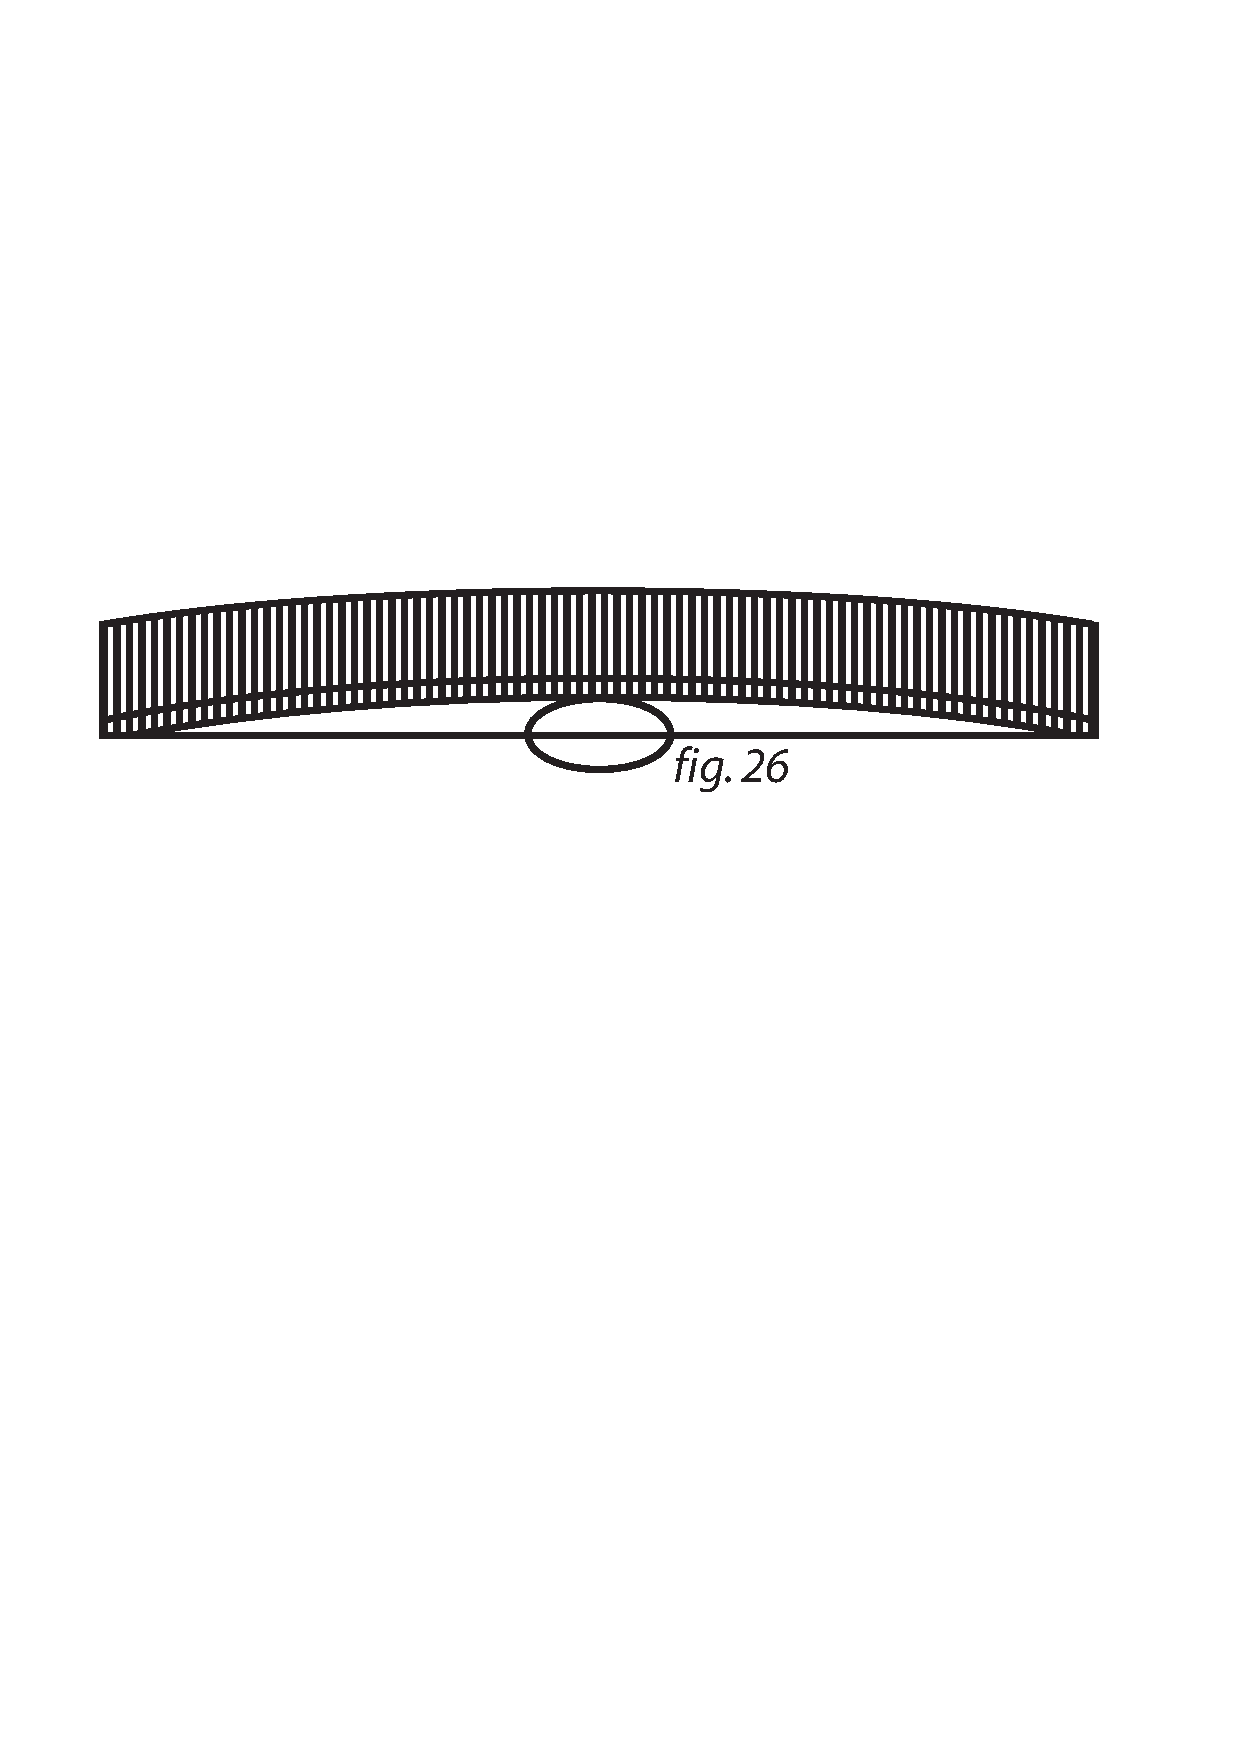
\includegraphics[trim = 0mm -1mm 0mm 0mm, clip, width=0.6\textwidth]{images/LH0351506_014r-d1.pdf}\\
\centering [\textit{Fig. 7, nach Hooke Fig. 26}]
\pend
\vspace{2.5em}
\setline{16}
\pstart
%\noindent
\centering
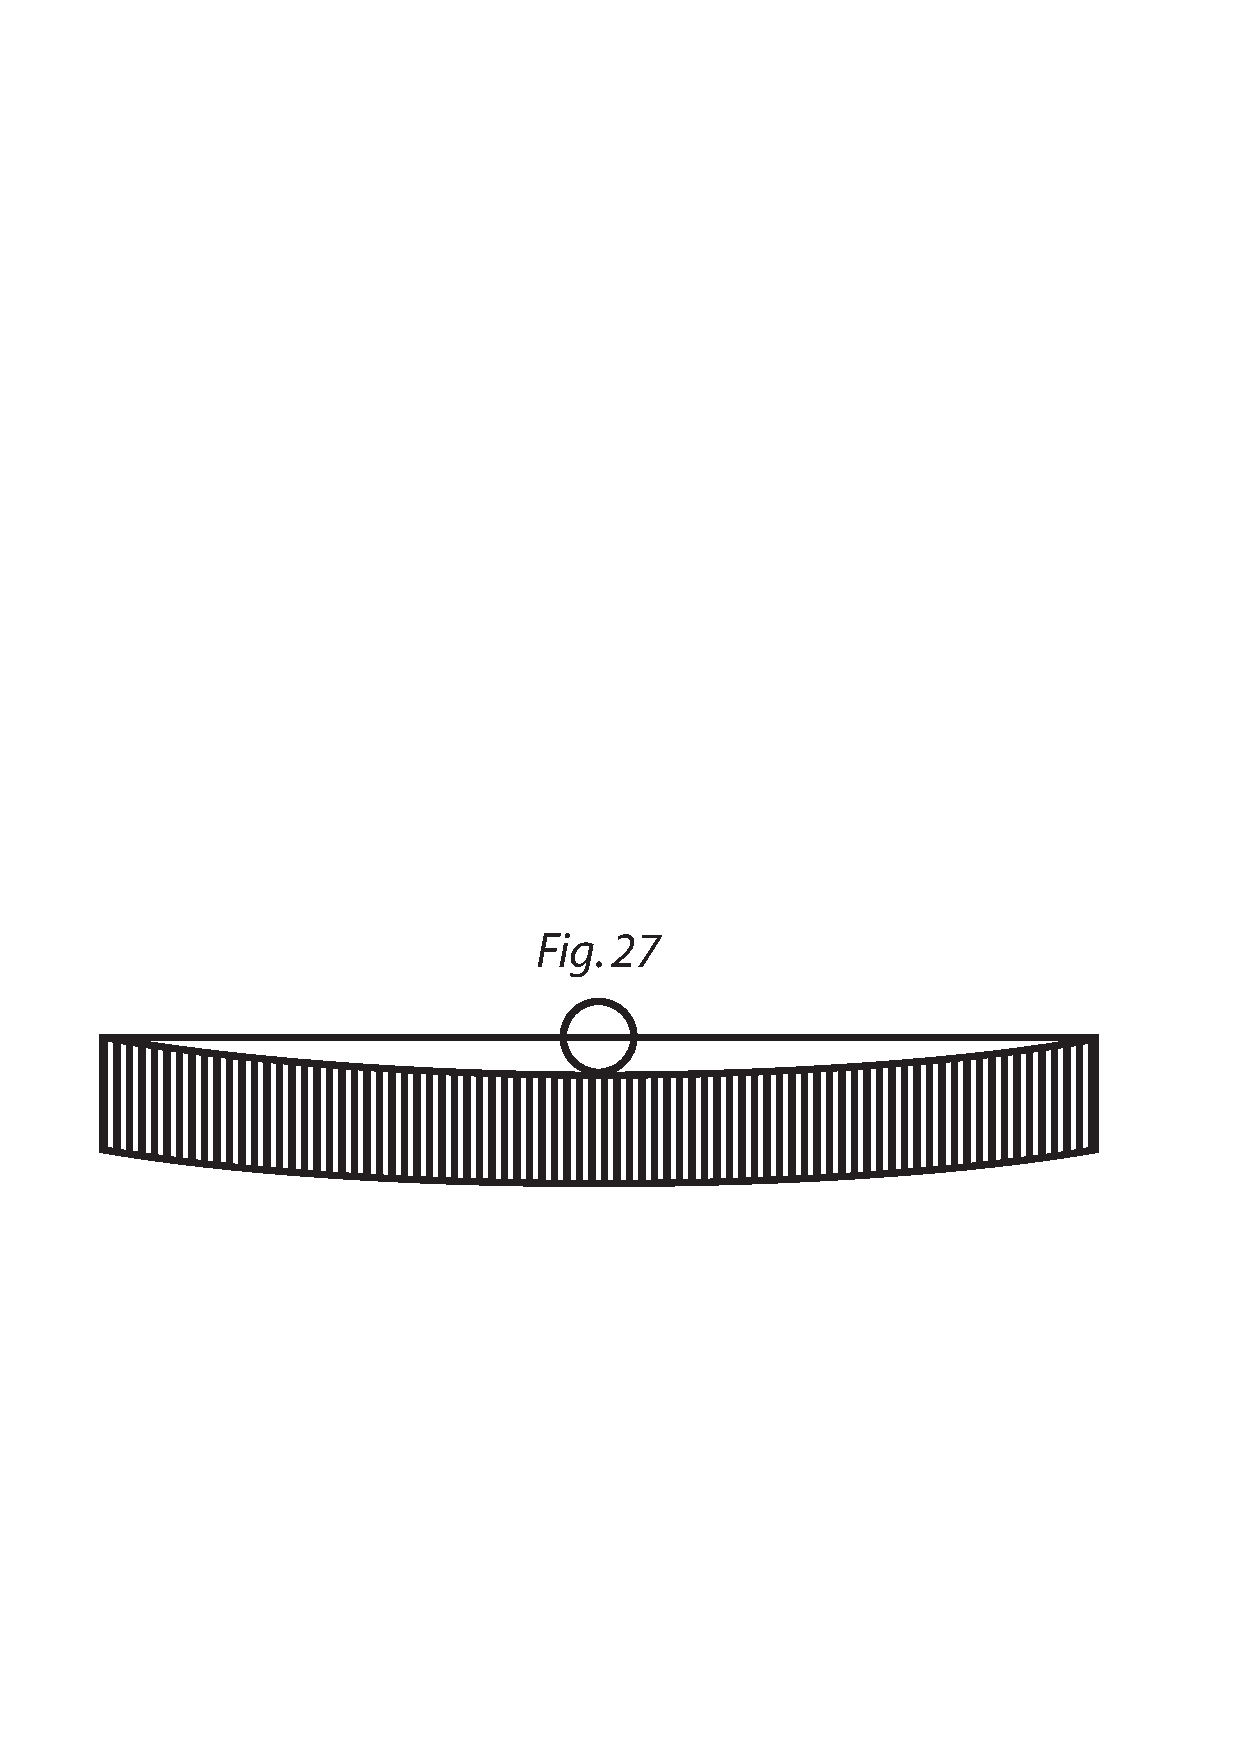
\includegraphics[trim = 0mm -4mm 0mm 0mm, clip, width=0.6\textwidth]{images/LH0351506_014r-dext27.pdf}\\
\centering [\textit{Fig. 8, erg. Hrsg. nach Hooke Fig. 27}]
%\end{center}
\pend
%\vspace{1em}
\newpage
\pstart \textit{The curvity of the said plate is express'd 26 fig.}\edtext{}{\lemma{\textit{fig}.}\Cfootnote{a.a.O., S. 65.}} Jam quicquid hac via fieri potest aqua et bullis aeris idem fieri potest \textit{with the same glasses turned upside-down,}\edtext{}{\lemma{\textit{upside-down},}\Cfootnote{a.a.O., S. 65.}} ope exacte rotundi et politi cylindri vel globuli vitrei, vel ex crystallo, \textit{cornelian, Agate,}\edtext{}{\lemma{\textit{Agate},}\Cfootnote{a.a.O., S. 65.}} aut alio lapide \textit{exceeding hard and close}\edtext{}{\lemma{\textit{close}}\Cfootnote{a.a.O., S. 65.}}. Modo in 27 figura repraesentato, quae est inversa tantum fig. 26\textsuperscript{tae}. Quod enim illic bulla aeris quae summum petit, id hic facit globus qui tendit ad imum, sed opus est tum ut globulus sit valde rotundus, tum ut concavitas tabulae sit exacte polita ac libera ab omni pulvere, alioquin posset fieri ut globulus vel cylinder in debito loco quiesceret. Non possum hic quin mentionem faciam curiosae admodum libellae a Christophoro Wrenno\protect\index{Namensregister}{\textso{Wren}, Christopher (1632-1723)} \edtext{inventae}{\lemma{inventae}\Cfootnote{Vgl. \textsc{R. Hooke} (a.a.O., S. 65), der von solch einem Instrument Wrens berichtet.}} pro sumendo horizonte \textit{every way in a Circle.}\edtext{}{\lemma{\textit{Circle}.}\Cfootnote{a.a.O., S. 65.}} Quod fit largo concavo tornato ac polito ex sphaera valde larga, \textit{and the limb of it ground and polisht on} \edtext{\textit{a flat}}{\lemma{\textit{on}}\Bfootnote{\textit{(1)}\ \textit{a very large sphere} \textit{(2)}\ \textit{a flat} \textit{L}}}\textit{, for}\edtext{}{\lemma{\textit{for}}\Cfootnote{a.a.O., S. 65.}} \edtext{nam horizontaliter locando}{\lemma{\textit{for}}\Bfootnote{\textit{(1)}\ \textit{by placing} \textit{(2)}\ nam horizontaliter locando \textit{L}}}, et exiguam Hydrargyri guttulam infundendo, facile erit ope hujus limbi politi verum horizontem detegere. Unam ego inconvenientiam reperio, quod Mercurius habet aliquod genus adhaesionis ad vitrum, sed exiguus globulus crystallinus malo mederi potest. 
\pend 
\pstart Quinta instrumenti excellentia est, quod summae illae inconvenientiae in movendo instrumento una cum objecto possunt evitari; instrumento objectum sua sponte sequente. \textit{I make an axis of very dry and strong dram-fir}\edtext{}{\lemma{\textit{dram-fir}}\Cfootnote{a.a.O., S. 67.}} \edtext{magnae satis crassitiei}{\lemma{\textit{dram-fir}}\Bfootnote{\textit{(1)}\ \textit{of a bigness} dig \textit{(2)}\ magnae satis crassitiei \textit{L}}} pro longitudine ne curvetur in inferiore ejus parte, figo in medio \edtext{[\textit{well bound and hoop'd about} (hoope, vieo, binder) \textit{with iron}]}{\lemma{[\textit{well ... iron}]}\Cfootnote{a.a.O., S. 67, eckige Klammern von Leibniz.}} centrum vel punctum chalybeum, valde bene tornatum duratum et acutum, quod moveatur in foramine conico apto ad ipsum recipiendum, etiam ex bono et durato chalybe: et ab altero latere hujus arboris vel virgae figo aliam chalybeam portionem in ipso medio, quod qua parte ligno immediate contiguum est, habet \textit{a Neck very well tourned and hardned, a little tapering from the wood outward, wich is to be moved in a collar fit for it, as i shal shew by and by, and at a convenient distance from the said neck, as at somewhat more then half the radius of the instrument, is made a cylindrical-neck, fitted with a collar of brass with a joynt and other apparatus, large enoug to carry the Table and Instrument firm and true, without sliding or yielding in its socket after it be once set. This axis by the collar and conical hole below, i place parallel to the axis, wich by some tryals is easely enoug adjusted; about the cylindrical Neck, at the upper end of this Axis, is a Socket of Brass, fastned with a screw, wich Socket claspeth in a joynt, a short arm, wich has at one end a Ball that is fitted into a socket,}
%\edtext{}{\lemma{socket,}\Cfootnote{a.a.O., S. 67.}} 